\chapter{Clasificación}

\section{Introducción}
Analizado el dataset Bupa, en este capítulo se desarrollan diferentes modelos predictivos utilizando la información obtenida previamente.
Se construirán modelos basados en k-NN (aplicado a la clasificación), modelos basados en LDA (Lineal Discriminant Analisys) y QDA (Quadratic Discriminant Analysis).\\


Importante: Tras la realización del EDA se ha optado por aplicar alguno de los cambios efectuados. Se han eliminado aquellas filas detectadas como repetidas, se ha eliminado la columna 'selector', y se han normalizado los datos.
El cambio más importante es que la variable dependiente, 'drinks', ha sido separada en dos clases tal y como se justifica en el apartado \ref{drinks}





\section{Utilizar el algoritmo k-NN probando con diferentes valores de k}
En primer lugar, se elaboran y estudian modelos de clasificación bastados en k-NN usando como métrica de rendimiento el Accuracy (precisión): la fracción de predicciones que el modelo realizó correctamente.
Se crearán diferentes modelos cada uno con un valor de k diferente.

\newpage
\begin{table}[!h]
	\resizebox{15cm}{!} {
	\begin{tabular}{l|lllllllllll}
		& Fold 1    & Fold 2    & Fold 3    & Fold 4    & Fold 5    & Fold 6    & Fold 7    & Fold 8    & Fold 9    & Fold 10   & Media     \\ \hline
		k=1  & 0.7058824 & 0.7352941 & 0.7000000 & 0.6969697 & 0.7647059 & 0.7058824 & 0.7647059 & 0.5588235 & 0.6060606 & 0.6764706 & 0.6914795 \\
		k=3  & 0.7647059 & 0.6764706 & 0.8333333 & 0.6363636 & 0.8529412 & 0.7647059 & 0.7647059 & 0.7647059 & 0.7575758 & 0.7352941 & 0.7550802 \\
		k=5  & 0.7647059 & 0.6764706 & 0.9000000 & 0.6060606 & 0.8529412 & 0.7352941 & 0.7941176 & 0.7352941 & 0.6969697 & 0.8235294 & 0.7585383 \\
		k=7  & 0.7647059 & 0.7941176 & 0.9000000 & 0.6666667 & 0.8529412 & 0.8235294 & 0.7941176 & 0.7647059 & 0.6969697 & 0.7058824 & 0.7763636 \\
		k=10 & 0.7352941 & 0.6764706 & 0.9000000 & 0.6969697 & 0.8529412 & 0.8235294 & 0.7352941 & 0.8823529 & 0.6969697 & 0.7352941 & 0.7735116 \\
		k=13 & 0.7647059 & 0.7352941 & 0.8666667 & 0.6363636 & 0.8529412 & 0.7941176 & 0.7352941 & 0.8823529 & 0.6969697 & 0.7941176 & 0.7758824 \\
		k=15 & 0.7647059 & 0.7352941 & 0.9333333 & 0.6666667 & 0.8823529 & 0.7941176 & 0.7941176 & 0.8529412 & 0.6969697 & 0.7941176 & \textbf{0.7914617} \\
		k=17 & 0.7941176 & 0.6764706 & 0.9333333 & 0.6666667 & 0.8823529 & 0.7941176 & 0.7352941 & 0.8529412 & 0.7272727 & 0.7941176 & 0.7856684 \\
		k=20 & 0.7647059 & 0.7352941 & 0.9000000 & 0.6363636 & 0.8823529 & 0.7941176 & 0.7352941 & 0.8529412 & 0.7272727 & 0.7941176 & 0.7822460 \\
		k=30 & 0.7352941 & 0.7058824 & 0.9000000 & 0.5757576 & 0.8823529 & 0.7941176 & 0.7058824 & 0.8823529 & 0.6969697 & 0.7941176 & 0.7672727
	\end{tabular}
}
\end{table}

Tras la ejecución de todos los casos, se observa que el modelo que ha obtenido el mejor rendimiento es aquel en el que el valor de k = 15, con una precisión del 79,1\%.


\vspace{1cm}
\section{Utilizar el algoritmo LDA para clasificar.}
En esta sección, se elaboran y estudian modelos de clasificacion bastados en LDA. Este tipo de modelo se realizan en base a una serie de asunciones, las cuales se deben garantizar para asegurar el correcto rendimiento del modelo.\\

La primera de estas asunciones se centra en la normalidad en las distribuciones de cada atributo. Como ya se observó durante la realización del análisis exploratorio \ref{anali}, el test de Shapiro-Wilk confirmó que no existe ninguna distribución normal dentro de los datos. \\

Otra asunción de este método es que todas las variables deben tener una varianza similar. Observemos en la siguiente tabla si es ese el caso:
\begin{table}[!h]
	\centering
	\begin{tabular}{l|l}
		Variables & Varianza     \\ \hline
		mcv       & 19.8237364   \\
		alkphos   & 339.7381922  \\
		sgpt      & 383.6211489  \\
		sgot      & 102.3241677  \\
		gammagt   & 1555.4645851
	\end{tabular}
\end{table}

Fácilmente se observa que no hay similitud entre estos valores.\\

Pese a no cumplir con las asunciones previas, se realiza el modelo LDA sin tener la garantía de correcto rendimiento del modelo. Para ello, se utiliza la función 'lda()' del paquete 'MASS'. Este método requiere especificar la variable a predecir y aquellas que se usarán para la predicción. Tanto en este caso como en el posterior modelo QDA se han utilizado todas las variables independientes para la predicción menos la variable 'selector'.

\newpage
Los resultados del modelo LDA sobre 10-folds:

\begin{table}[!h]
	\resizebox{15cm}{!} {
	\begin{tabular}{l|lllllllllll}
		& Fold 1    & Fold 2    & Fold 3    & Fold 4    & Fold 5    & Fold 6    & Fold 7    & Fold 8    & Fold 9    & Fold 10   & Media     \\ \hline
		Accuracy & 0.7058824 & 0.7352941 & 0.8666667 & 0.6363636 & 0.8235294 & 0.7941176 & 0.7058824 & 0.8823529 & 0.7575758 & 0.7941176 & 0.7701783
	\end{tabular}
}
\end{table}










\vspace{1cm}
\section{Utilizar el algoritmo QDA para clasificar.}
Finalmente, se elaboran y estudian modelos de clasificación bastados en QDA.
Respecto a las asunciones de QDA son similares a las de LDA, la única diferencia es que la similitud de las varianzas de cada variable se debe tener en cuenta respecto a cada clase a predecir. Para comprobar si se cumple, se utiliza el test de Levene:
\begin{table}[!h]
	\centering
	\begin{tabular}{l|lll}
		Variables & Df & F value & Pr(\textgreater{}F) \\ \hline
		mcv       & 1  & 0.0391  & 0.8434              \\
		alkphos   & 1  & 2.8435  & 0.09266             \\
		sgpt      & 1  & 10.646  & 0.001215            \\
		sgot      & 1  & 4.3484  & 0.03779             \\
		gammagt   & 1  & 15.386  & 0.0001061          
	\end{tabular}
\end{table}

Se observa que exceptuando el caso de la variable 'mcv', el resto no llega a un valor de p-value que supere el nivel de significancia (0.05), por lo tanto se rechaza la hipótesis nulas, confirmando que existen diferencia significativas entre las varianzas.\\

Otra de las asunciones de este modelo es la ausencia de niveles de correlación entre las distintas variables para cada clase. Se observan estos niveles de correlación mediante el coeficiente de Kendall para cada una de las dos clases:

\newpage
\begin{figure}[!tbh]
	\centering
	\begin{subfigure}{0.5\textwidth}
	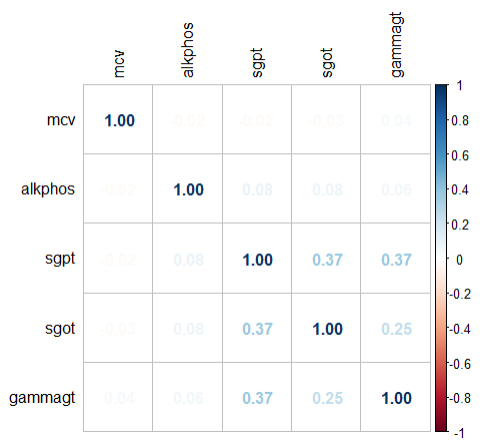
\includegraphics[width=1\linewidth]{figures/corr_0}
\caption{drinks = 0}
\label{fig:corr0}
	\end{subfigure}\hfil % <-- added
	\begin{subfigure}{0.5\textwidth}
	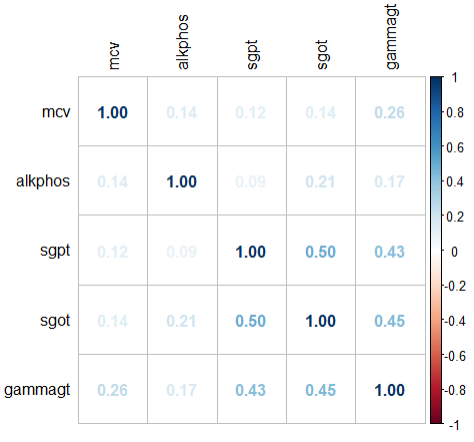
\includegraphics[width=1\linewidth]{figures/corr_1}
\caption{drinks = 1}
\label{fig:corr1}
	\end{subfigure}\hfil % <-- added
\end{figure}



En ambos casos se observa que los niveles de correlación son bajos en prácticamente todos los casos, por lo que esta asunción si se cumple.\\

Para ejecutar QDA se utiliza la función 'qda()' de la librería 'MASS' y una vez más se utilizan todas las variables independientes para predecir la dependiente, menos la variable 'selector'. \\

Obtenemos los siguientes resultados sobre 10-folds:
\begin{table}[!h]
	\resizebox{15cm}{!} {
	\begin{tabular}{l|lllllllllll}
		& Fold 1    & Fold 2    & Fold 3    & Fold 4    & Fold 5    & Fold 6    & Fold 7    & Fold 8    & Fold 9    & Fold 10   & Media     \\ \hline
		Accuracy & 0.7352941 & 0.6764706 & 0.9000000 & 0.4848485 & 0.8235294 & 0.7941176 & 0.7058824 & 0.7941176 & 0.7272727 & 0.7647059 & 0.7406239
	\end{tabular}
}
\end{table}




\newpage
\section{Comparar los resultados de los tres algoritmos}
Los tres algoritmos han dado lugar a resultados bastantes similares, respecto al valor de precisión generado. El mejor resultado ha sido obtenido con el algoritmo knn con un número de k = 15. Justificando unos inferiores resultados con LDA se debe partir de que no se han cumplido las asunciones que acompañan a este algoritmo lo que explica el peor rendimiento de este algoritmo. De forma similar ocurre con QDA, en ambos casos se añade el factor de que no tenemos el suficiente número de casos en cada clase.

\begin{table}[!h]
	\centering
	\begin{tabular}{l|lll}
		& knn (k=15) & LDA       & QDA       \\ \hline
		Accuracy & 0.7914617  & 0.7701783 & 0.7406239
	\end{tabular}
\end{table}

Aunque se haya alcanzado una precisión superior al 70\% en todos los casos, se debe recordar que partimos de un problema balance entre el número de casos para cada una de las dos clases, lo cual se traduce en una peor clasificación la clase con menor número de casos iniciales.\\


Se finaliza con la aplicación del test de Friedman para determinar si realmente existen diferencias significativas entre los tres modelos creados. Para ello, se toman los valores de precisión resultantes para cada modelo aportado por el profesorado. En ese mismo archivo modificaremos los resultados sobre el dataset tratado, 'Bupa', para que contenga los resultados de los algoritmos efectuados a los largo de este proyecto.

Friedman rank sum test
\begin{table}[!h]
	\centering
	\begin{tabular}{lll}
		chi-squared & df & p-value \\ \hline
		0.7      & 2  & 0.7047
	\end{tabular}
\end{table}

Obteniendo un p-value superior al nivel de significancia no es posible rechazar la hipótesis nula de que los tres modelos evaluados presenten similitud entre ellos. En definitiva, se concluye en que los tres modelos generados ofrecen resultados similares sobre el conjunto de datos trabajado.













